

\chapter{Decision Making}

\section{Introduction}

Conditional statements and decision making plays an important role in algorithmic design. In this chapter, we see how an condition statment can be implemented, and what is the corresponding hardware for such a task.

\section{Recap}

Recall that a condition is usually implemented in software as \verb|if-else| as shown in \autoref{fig:conditions:condition_soft}.


\begin{figure}[h]
\centering
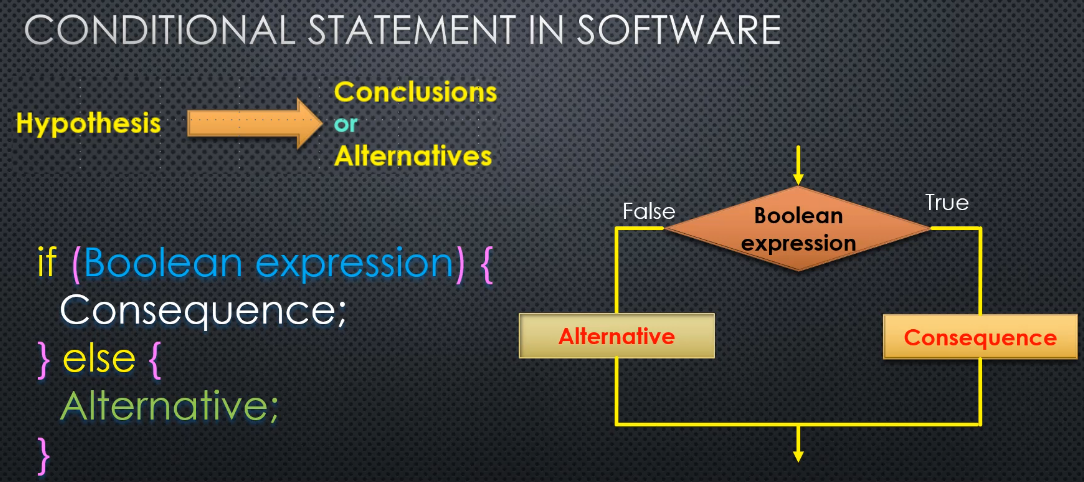
\includegraphics[scale=0.35,frame]{Figures/conditions/condition_soft}
\caption{Condition in software}
\label{fig:conditions:condition_soft}
\end{figure}

\begin{itemize}

\item We have some condition define by some boolean expression

\item if the condition is true consequence is selected else the alternative is selected

\end{itemize}

\newpage
As hardware, and \verb|if-else| statement can be modeled using a switch as shown in 

\begin{figure}[h]
\centering
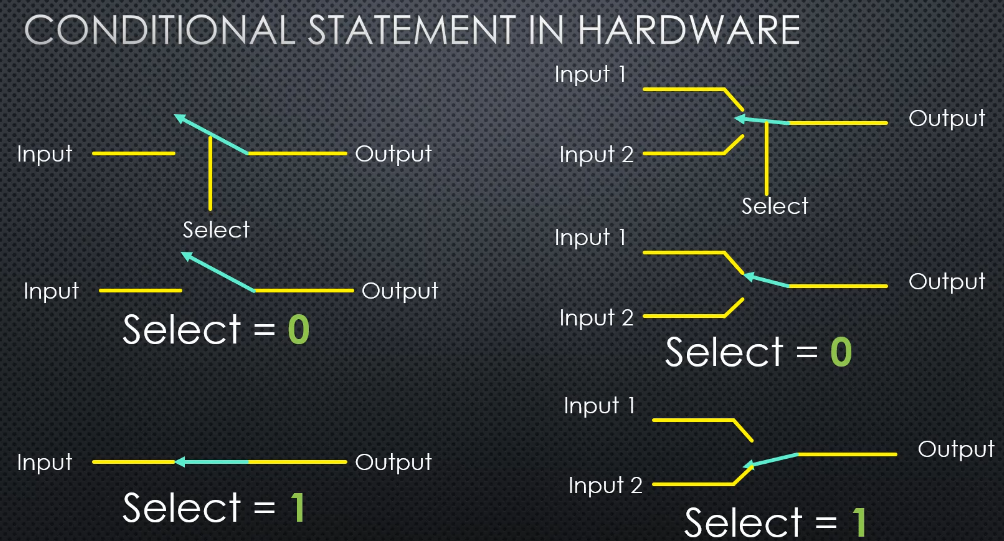
\includegraphics[scale=0.35,frame]{Figures/conditions/condition_hard_switch}
\caption{Condtion modeled using a switch}
\label{fig:conditions:condition_hard_switch}
\end{figure}

\begin{itemize}

\item In the special case we have switch to select between 1 input

	\begin{itemize}
	\item This correspond to a special \verb|if| where we have no  \verb|else| condition
	\end{itemize}

\item Then the general case where switch is selecting between multiple inputs

\end{itemize}



\newpage
\section{Multiplexer}

To impelement conditions using logic gates, usually we use a MUX circuit as shown in \autoref{fig:conditions:MUX}.

\begin{figure}[h]
\centering
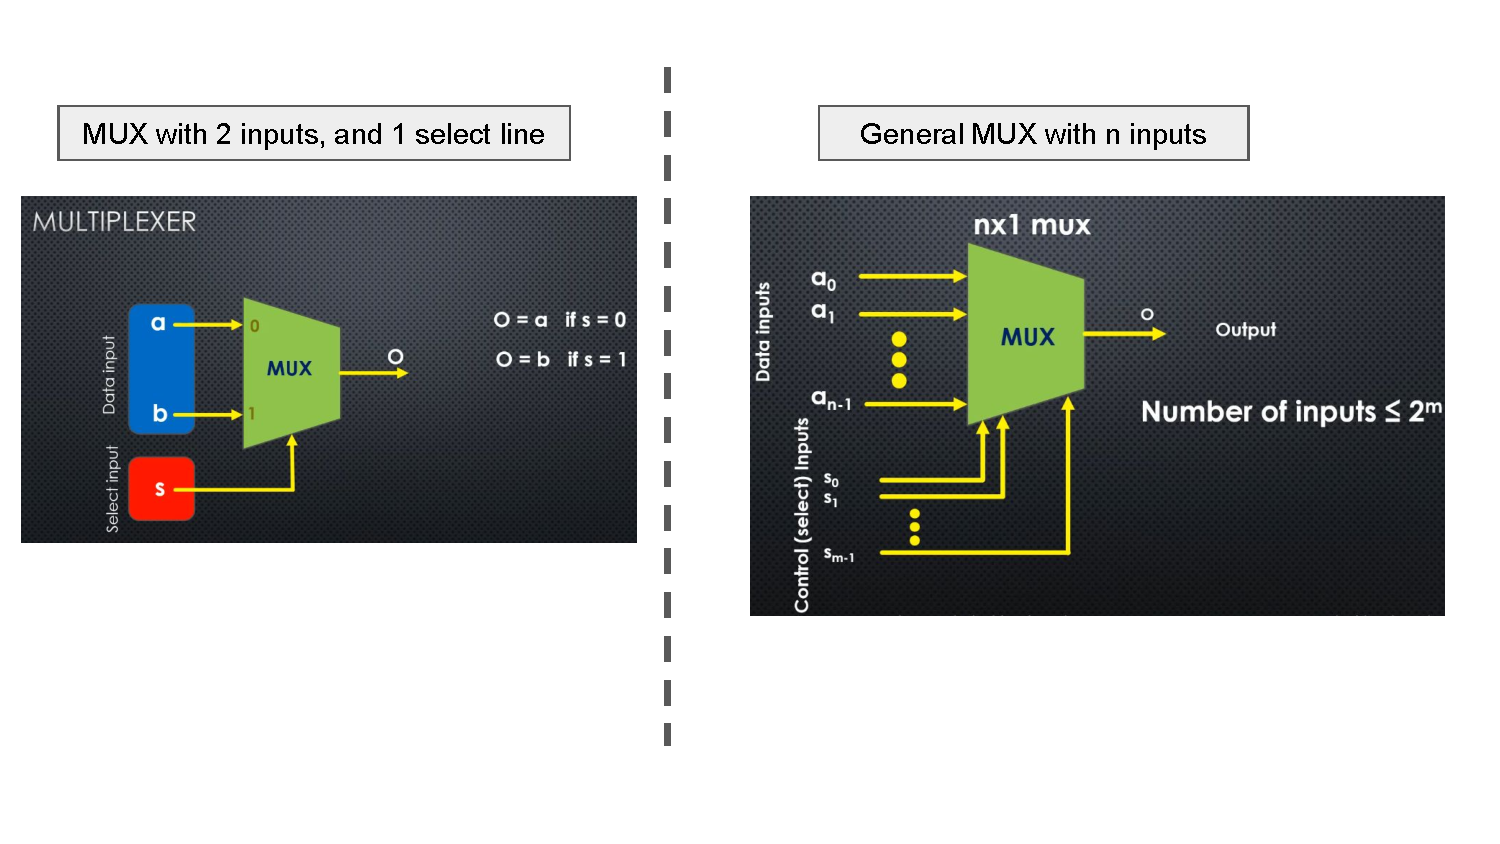
\includegraphics[scale=0.65,frame]{Figures/conditions/MUX}
\caption{Multiplexer}
\label{fig:conditions:MUX}
\end{figure}

\begin{itemize}

\item In the right hand side, we have the special case MUX where we have 1 select line to select between inputs

\item Then we have the generalize case where we have $m$ select line to select between $n$ inputs

\end{itemize}

\newpage
\subsection{Generalized Mux and if-else}

Now in real applications, the MUX shown in \autoref{fig:conditions:MUX} doesn't come in straightforward manner, we usually apply some preprocessing steps on the selection line or even in the input section, to have the appropriate output.

\begin{figure}[h]
\centering
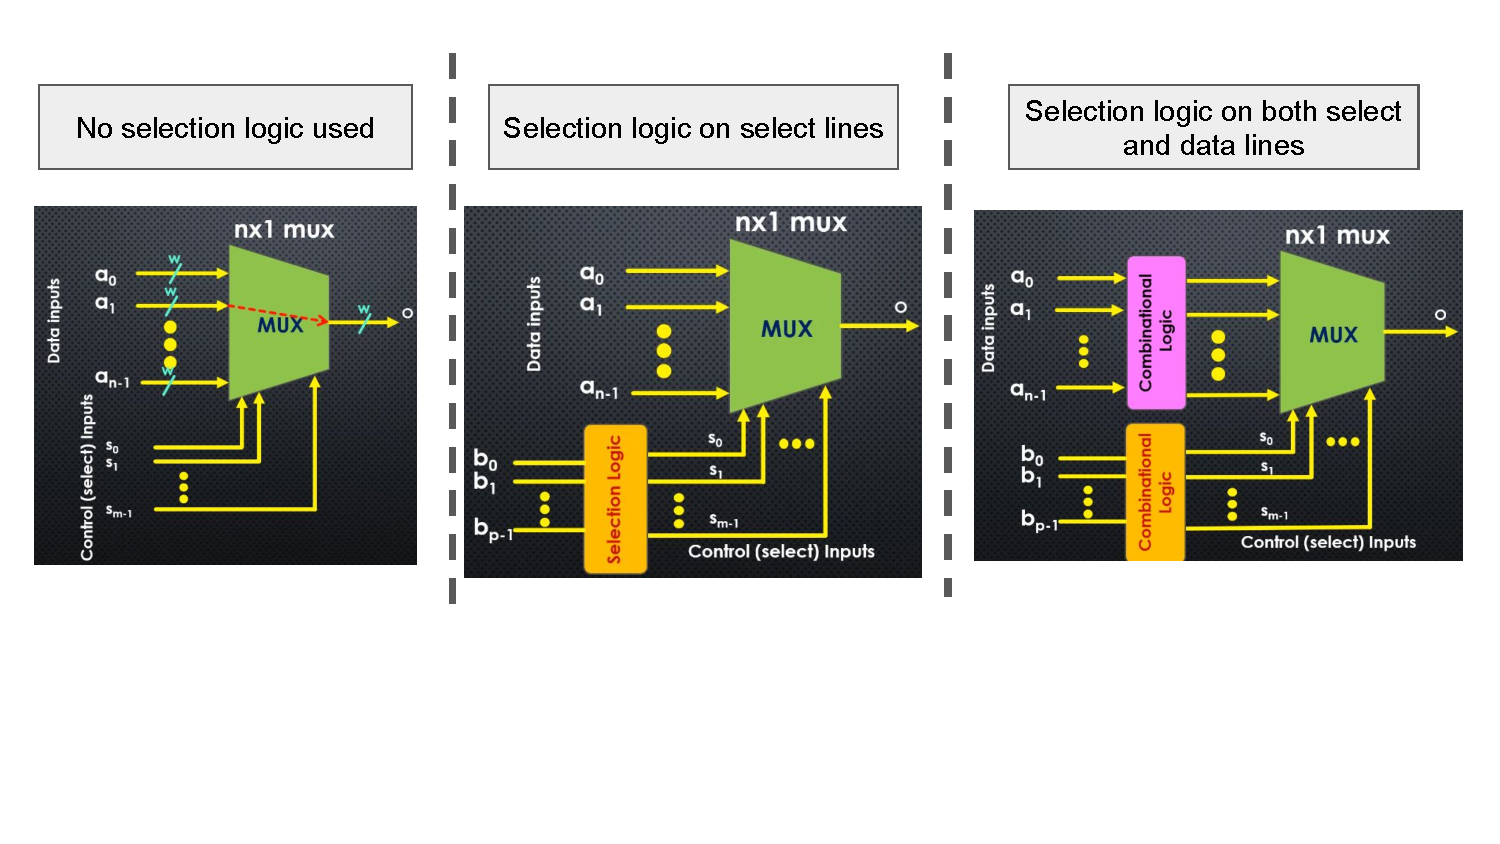
\includegraphics[scale=0.65,frame]{Figures/conditions/generalized_mux}
\caption{Generalized Multiplexer Circuits}
\label{fig:conditions:generalized_mux}
\end{figure}


We see in this section some examples to see the mapping between \verb|if-else| conditions and the corresponding MUX circuit.

\newpage
$\mathrm{1}^\mathrm{st}$ example is presented in \autoref{fig:conditions:if_else_ex_1}

\begin{figure}[h]
\centering
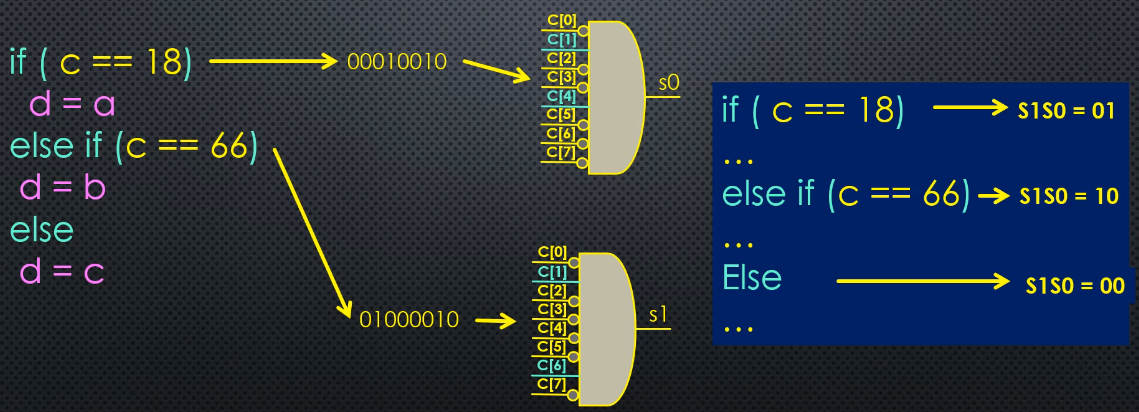
\includegraphics[scale=0.35,frame]{Figures/conditions/if_else_ex_1}
\caption{if esle example}
\label{fig:conditions:if_else_ex_1}
\end{figure}

\begin{itemize}

\item We have on the right hand side some \verb|if-else| statment

	\begin{itemize}
	\item \verb|d| is output, \verb|a|,\verb|b| and \verb|c| inputs
	
	\item \verb|c| is also present the role of the selection line
	\end{itemize}

\item Here we need to select line $s_0$ and $s_1$ since we have 4 inputs

\item the conditions \verb|c==18| and \verb|c==66| are mapped to some \verb|AND| gate, each with their corresponding binary values

\item When $s_1 \, s_0 \, = \, 01$ condition \verb|c==18| is validate, hence \verb|a| is selected and mapped to output \verb|d|, and same logic with other values

\end{itemize}

The corresponding MUX circuit of \autoref{fig:conditions:if_else_ex_1} is shown in \autoref{fig:conditions:if_else_ex_1_circuit}.

\begin{figure}[h]
\centering
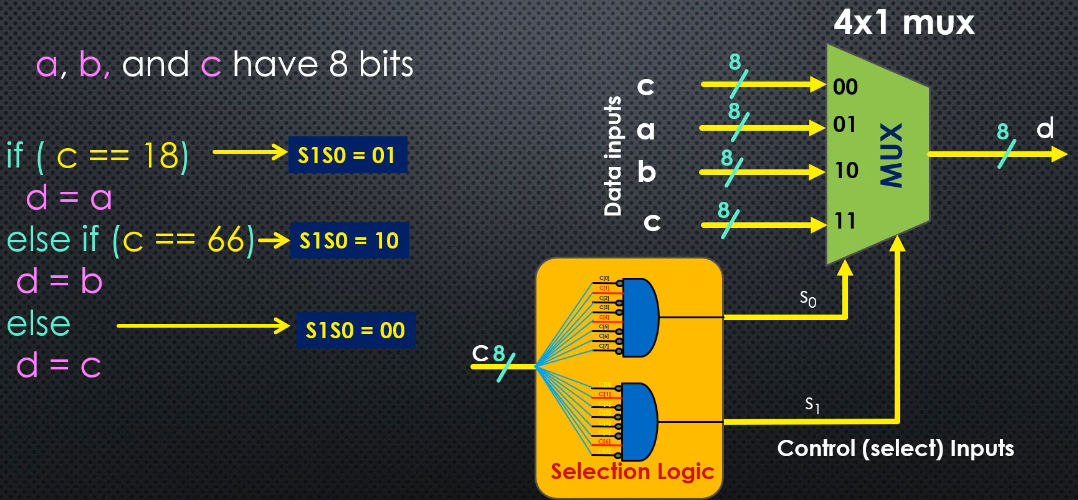
\includegraphics[scale=0.35,frame]{Figures/conditions/if_else_ex_1_circuit}
\caption{if esle example with MUX circuit}
\label{fig:conditions:if_else_ex_1_circuit}
\end{figure}

\newpage
$\mathrm{2}^\mathrm{nd}$ example is presented in \autoref{fig:conditions:if_else_ex_2}, where combinational logic are also presented on the input line section, since we have some preprocessing before passing inputs to output line \verb|d|

\begin{figure}[h]
\centering
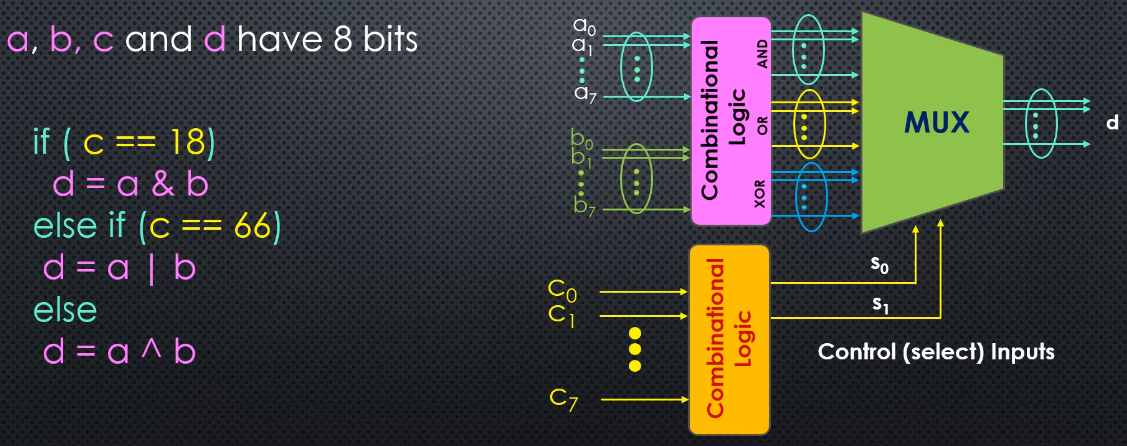
\includegraphics[scale=0.35,frame]{Figures/conditions/if_else_ex_2}
\caption{if esle example: combinational circuit on both lines}
\label{fig:conditions:if_else_ex_2}
\end{figure}

\newpage
\subsection{Quiz}

\underline{Quiz 1:} what is the hardware implementation that implement decision making process shown in \autoref{fig:conditions:quiz_if_else}?

\begin{figure}[h]
\centering
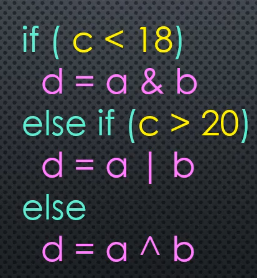
\includegraphics[scale=0.45,frame]{Figures/conditions/quiz_if_else}
\caption{Quiz 1}
\label{fig:conditions:quiz_if_else}
\end{figure}

\underline{Solution Quiz 1:}

\begin{figure}[h]
\centering
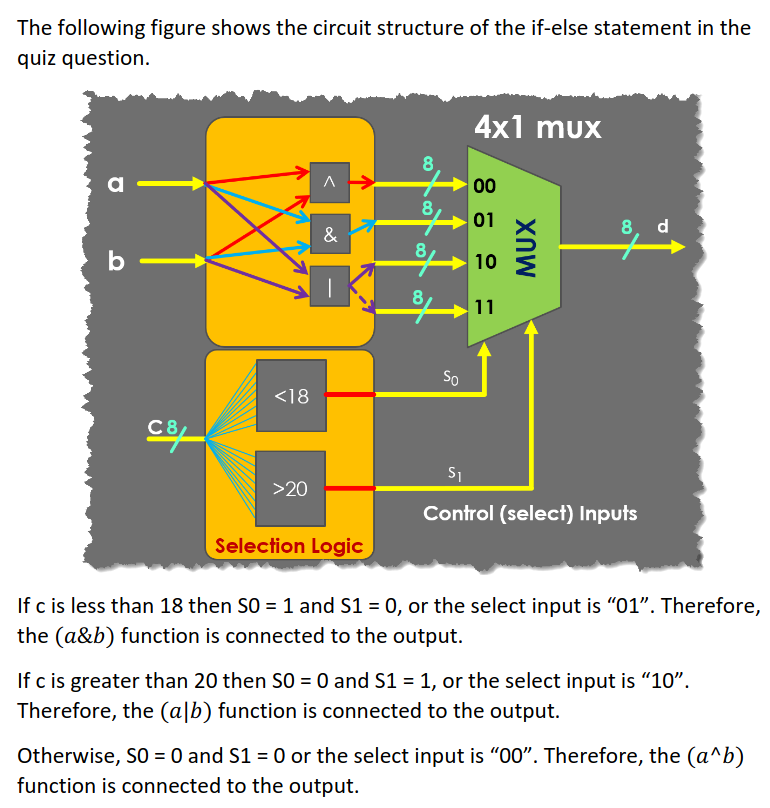
\includegraphics[scale=0.40,frame]{Figures/conditions/quiz_if_else_sol}
\caption{Quiz 1 Solution}
\label{fig:conditions:quiz_if_else_sol}
\end{figure}

\newpage
\underline{Quiz 2:} Draw the structure of the combinational circuit that can implement the \verb|HLS| code shown in \autoref{fig:conditions:quiz_switch_case}.

\begin{figure}[h]
\centering
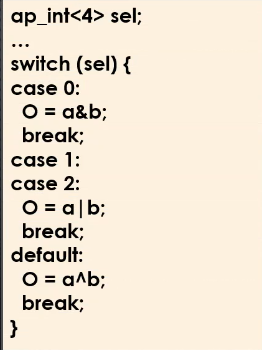
\includegraphics[scale=0.35,frame]{Figures/conditions/quiz_switch_case}
\caption{Quiz 2}
\label{fig:conditions:quiz_switch_case}
\end{figure}

\underline{Solution Quiz 2:}

\begin{figure}[h]
\centering
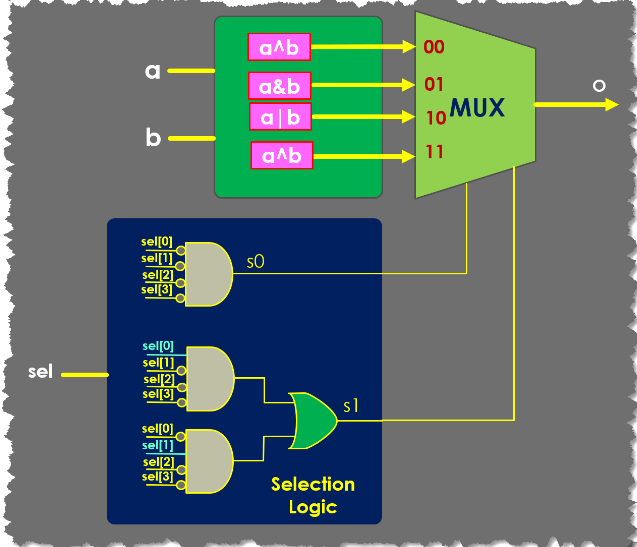
\includegraphics[scale=0.45,frame]{Figures/conditions/quiz_switch_case_sol}
\caption{Quiz 2 Solution}
\label{fig:conditions:quiz_switch_case_sol}
\end{figure}


\newpage
\section{Coders}

Now we move to coders circuit, that is encoder and decoder.

Recall that encoder is a circuit which transforms data from one shape to the other for various reason (security,compression,$\cdots$). Decoder does the opposite, that is retreive the original data from the coded data. In other words, encoders and decoders are circuit \tbi{change the forme of the data}.


\begin{figure}[h]
\centering
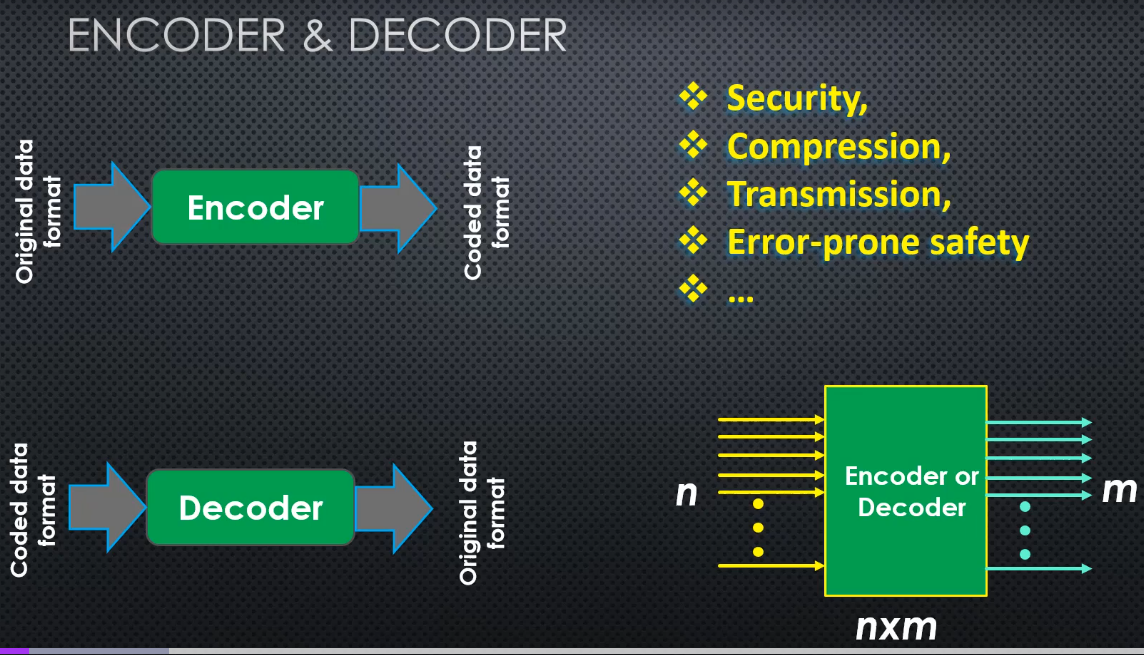
\includegraphics[scale=0.40,frame]{Figures/conditions/coders}
\caption{Encoder and Decoder}
\label{fig:conditions:coders}
\end{figure}


In general, coders circuit take $n$ input bits and generate $m$ output bits.

\newpage
\subsection{Examples}

As example, \autoref{fig:conditions:4_by_2_encoder} presents a 4 by 2 encoder. The encoder alwyas encode the input data \tbi{into a compact form}, so the number of output is less than the number of inputs.

\begin{figure}[h]
\centering
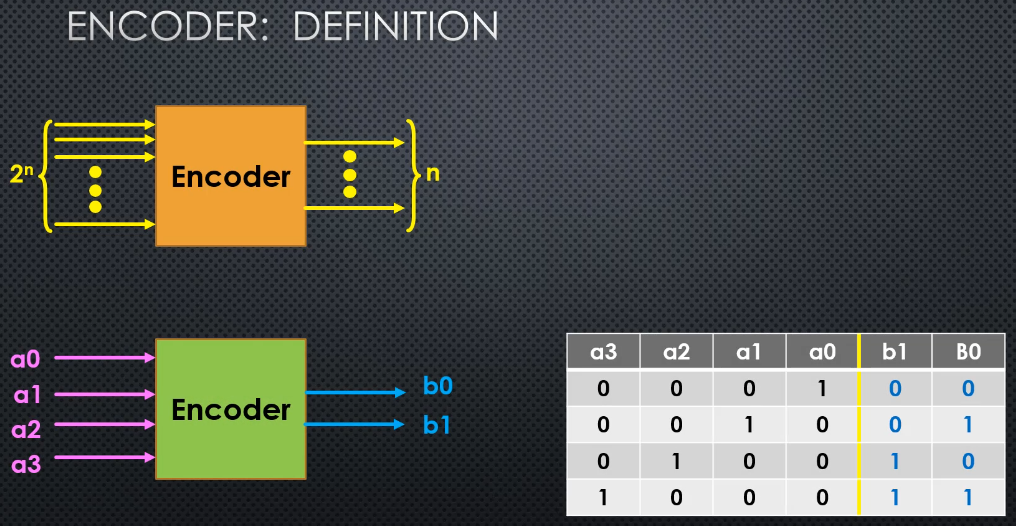
\includegraphics[scale=0.40,frame]{Figures/conditions/4_by_2_encoder}
\caption{4 by 2 Encoder}
\label{fig:conditions:4_by_2_encoder}
\end{figure}

The opposite of system in \autoref{fig:conditions:4_by_2_encoder} is presented in \autoref{fig:conditions:2_by_4_decoder}. Notice that binary input represents the position index of the 1 in output. For example last row , binary input 11 (equivalent to 3 in base 10) is the index of 1 in $b_0 \,b_1 \, b_2 \, b_3$

\begin{figure}[h]
\centering
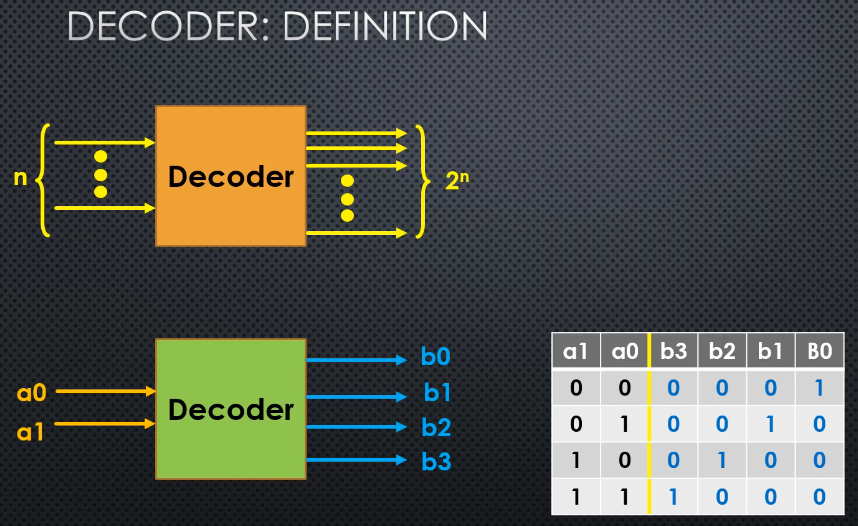
\includegraphics[scale=0.40,frame]{Figures/conditions/2_by_4_decoder}
\caption{2 by 4 Decoder}
\label{fig:conditions:2_by_4_decoder}
\end{figure}

\newpage
\subsection{Decoder in HLS}

An \verb|switch| case can be used to impelement a decoder or encoder in \verb|HLS|. The \verb|HLS| implementation of example of \autoref{fig:conditions:2_by_4_decoder} (the 2 by 4 decoder) is shown in \autoref{fig:conditions:2_by_4_decoder_hls}.


\begin{figure}[h]
\centering
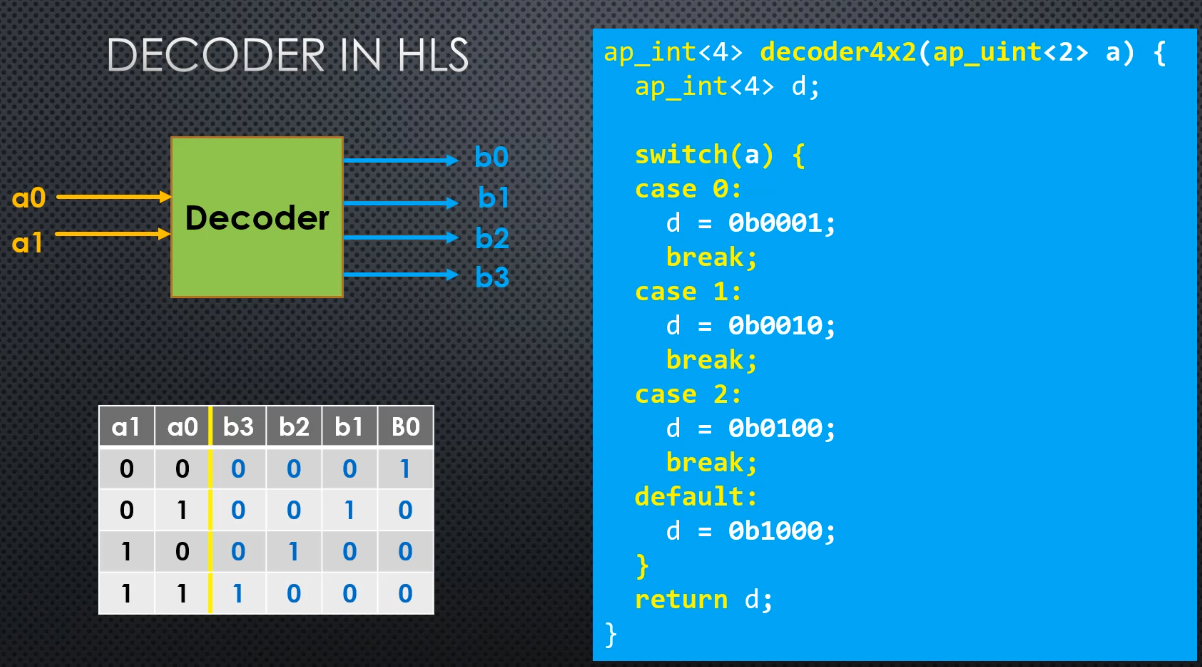
\includegraphics[scale=0.33,frame]{Figures/conditions/2_by_4_decoder_hls}
\caption{HLS impelemtation for 2 by 4 Decoder}
\label{fig:conditions:2_by_4_decoder_hls}
\end{figure}

The \verb|HLS| tool can the sythesise the code. A MUX can be used to implement the \verb|switch| case for the decoder as shown in \autoref{fig:conditions:2_by_4_decoder_hls_synthesis}.

\begin{figure}[h]
\centering
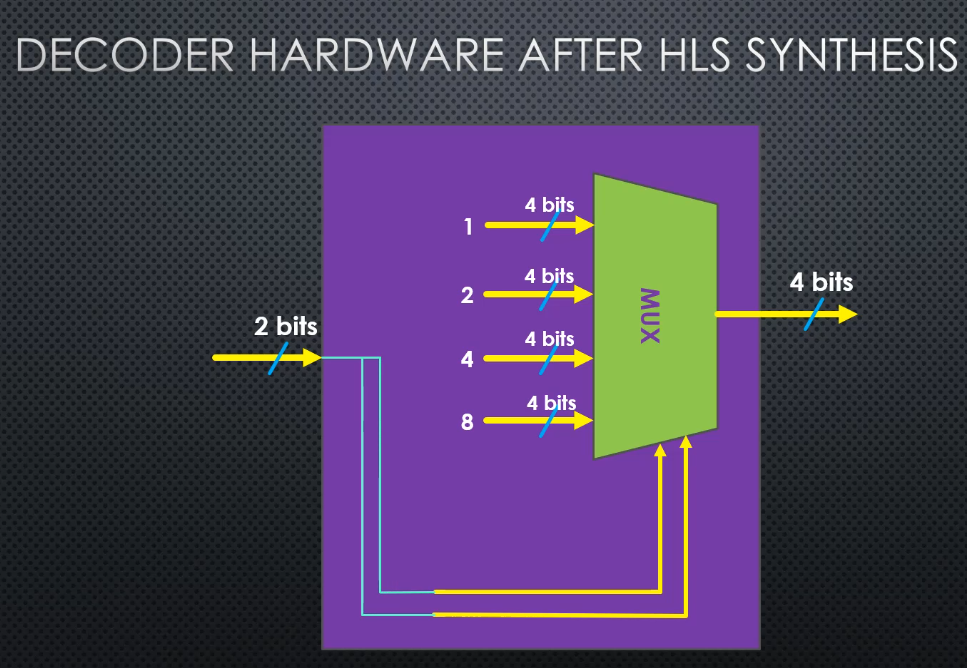
\includegraphics[scale=0.30,frame]{Figures/conditions/2_by_4_decoder_hls_synthesis}
\caption{HLS Synthesis for the 2 by 4 Decoder}
\label{fig:conditions:2_by_4_decoder_hls_synthesis}
\end{figure}


\newpage
\subsection{Quiz}

\underline{Quiz Decoder:} use a \verb|switch| case statement to describe and $8 \times 3$ encoder circuit.\\

\underline{Solution:}

\begin{figure}[h]
\centering
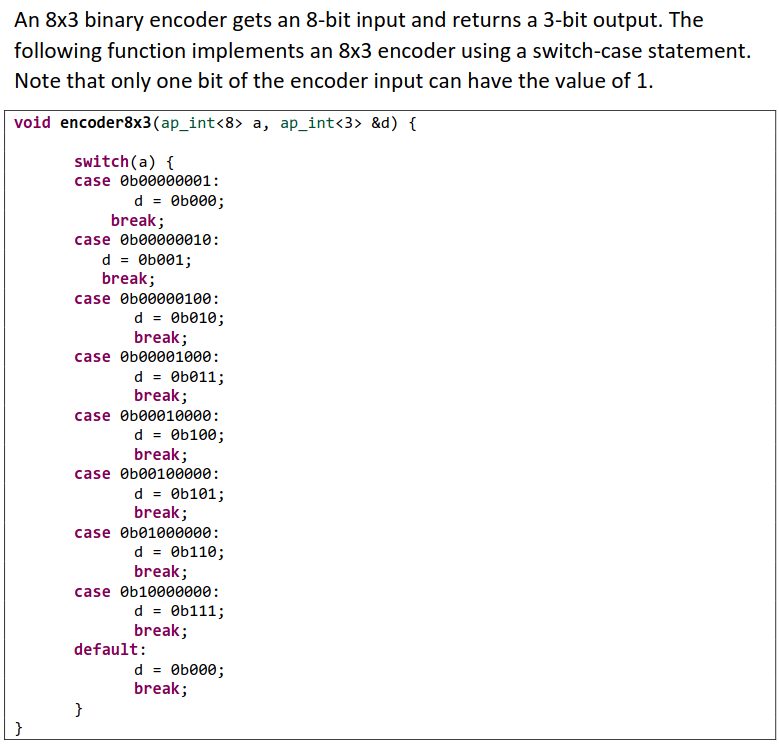
\includegraphics[scale=0.50,frame]{Figures/conditions/quiz_decoder}
\caption{Solution for quiz decoder}
\label{fig:conditions:quiz_decoder}
\end{figure}










